\chapter{Aspetti statistici delle misure}
	La \de{misura} è il valore numerico pari al rapporto tra una grandezza e un'altra ad essa omogenea assunta convenzionalmente come unità. Empiricamente l'operazione di misura fornisce un valore numerico non prevedibile a priori e non ripetibile: essa infatti comprende sempre un contributo \de{stocastico}, ossia casuale.
	
\section{Statistica descrittiva}
	La \de{statistica descrittiva} è un'insieme di tecniche, grafiche e matematiche, che permettono di descrivere il comportamento di una variabile \textbf{stocastica} (causale/aleatoria).
	
	\paragraph{Popolazioni e campioni} La \de{popolazione} rappresenta l'intero insieme, finito o infinito, di tutte le \textbf{possibili osservazioni}. 
	\begin{nota}
		La formulazione di \textit{finito} o \textit{ infinito} non ha una valenza matematica ma più \textit{pratica}.
	\end{nota} 
	
	Un \de{campione} è invece un sottoinsieme \textit{estratto a caso} dalla popolazione; esso può essere estratto con o senza reinserimento dall'insieme di partenza da cui nasce la definizione di
	\begin{itemize}
		\item \textbf{campionamento casuale semplice}, ossia ogni elemento estratto viene reinserito nella popolazione; questa modalità introduce la possibilità di estrarre due volte lo stesso elemento, tuttavia se il numero di campioni $n$ è molto minore della popolazione $N$ ($n\ll N$), tale probabilità è irrisoria;
		\item \textbf{campionamento in blocco}, ossia ogni elemento estratto riduce la popolazione rimanente in quanto non viene reinserito; questo metodo di estrazione è utile se la dimensione dei campioni $n$ è confrontabile con la dimensione della popolazione $N$ ($n\simeq N$).
	\end{itemize}
	
	\begin{esempio}{: popolazione e campioni}
		Un esempio di \textbf{popolazione} è l'insieme di tutti i perni prodotti da un impianto (in un periodo di tempo determinato) con le relative misure di diametro. Un sottoinsieme finito di $n$ elementi estratti a caso dalla popolazione rappresenta un \textbf{campione} della stessa.
	\end{esempio}
	
	\paragraph{Frequenza e probabilità} Dall'analisi del campione è possibile definire la \de{frequenza} della variabile aleatoria come il numero di volte che si osserva un determinato valore rispetto ad un certo numero di osservazioni. La \de{probabilità} rappresenta  il rapporto tra la frequenza e il numero di osservazioni effettuate.
	
	La \de{variabile} $x$ è detta \de{discreta} (e si indica con $x\in \mathds I$ se essa può assumere dei valori discreti, e in generale determinarne la frequenza è facile, mentre è detta \de{continua} (indicata con $x\in \mathds R$) se  la probabilità di avere valori duplicati tende a zero in quanto la variabile cambia con continuità.
		
	Per aggirare questo problema si raggruppano i dati raccolti in \de{classi} (in inglese \textit{bins}), ossia intervalli contigui di ampiezza nota e non necessariamente costante. A questo punto è possibile stabilire quante osservazioni della variabile aleatoria rientrano in ciascuna classe. La \de{probabilità} di ogni classe rappresenta dunque il rapporto tra osservazioni nella classe e le osservazioni totali misurate. La \de{densità di probabilità} rappresenta invece la probabilità divisa per l'ampiezza della sua classe.
	
	\subsection{Istogrammi} 
		Una volta che sono note frequenza (o conteggio), densità di frequenza, probabilità e relativa densità è possibile creare degli \de{istogrammi}, mostrati in figura \ref{fig:stat:istogrammi}, ossia dei grafici che permettono di osservare \textit{ad occhio} il valore dei risultati ottenuti.
	
		\begin{figure}[bht]
			\centering
			\begin{subfigure}{0.45\linewidth}
				\centering
				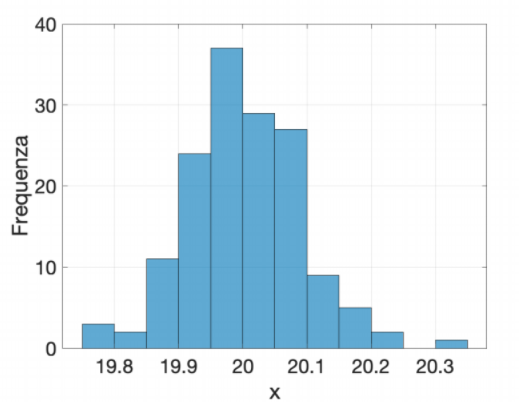
\includegraphics[width=5cm]{isto-a} \caption{}
			\end{subfigure}
			\begin{subfigure}{0.45\linewidth}
				\centering
				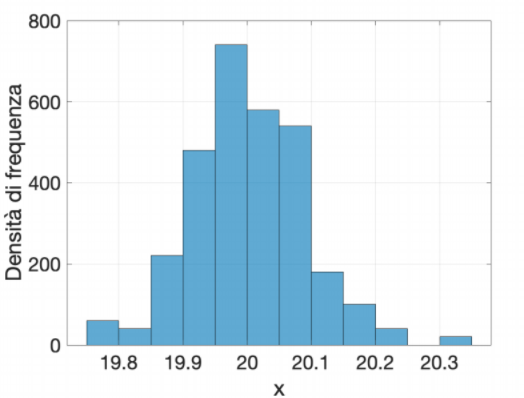
\includegraphics[width=5cm]{isto-b} \caption{}
			\end{subfigure}
			\begin{subfigure}{0.45\linewidth}
				\centering
				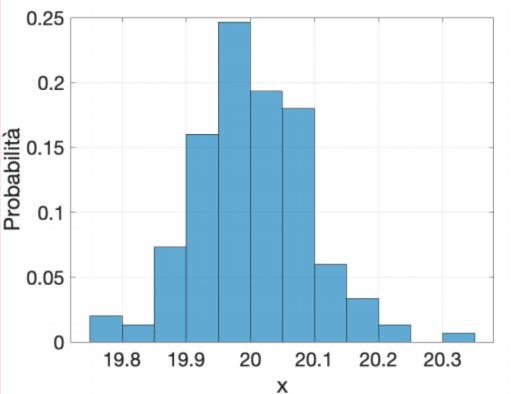
\includegraphics[width=5cm]{isto-c} \caption{}
			\end{subfigure}
			\begin{subfigure}{0.45\linewidth}
				\centering
				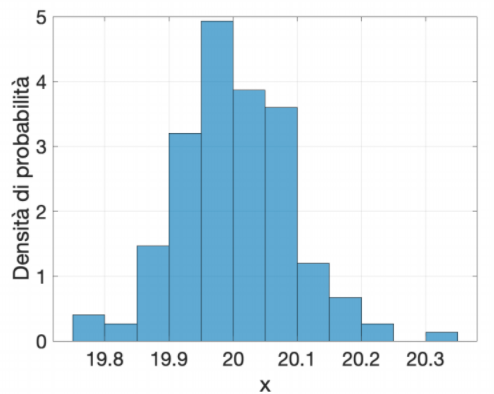
\includegraphics[width=5cm]{isto-d} \caption{}
			\end{subfigure}
			\caption{istogramma di frequenza (a), densità di frequenza (b), probabilità (c) e densità di probabilità (d) delle misurazioni di uno stesso campione. } \label{fig:stat:istogrammi}
		\end{figure}
		
		Il numero di classi (e la loro ampiezza) è in generale arbitraria e può non essere omogeneo; tuttavia è possibile utilizzare le cosiddette \de{formule di \textit{binning}} per stabilire il numero \textit{ideale} di classi $n$ da rappresentare in funzione del numero di campioni $N$:
		\begin{align*}
			\textrm{eq. di Scott:} & \qquad n = 3.5 s_x N^{-1/3} \\
			\textrm{eq. di Sturges:}& \qquad n = \lceil{1 + \log_2(N) \rceil}
		\end{align*}
		In queste relazioni il termine $s_x$ rappresenta la deviazione standard del campione analizzato.
		
		\paragraph{Diagramma cumulato} Un numero alternativo di rappresentare i dati tramite la cumulazione delle classi precedenti, come si può osservare in figura \ref{istocum}. Ogni \textit{canna} rappresenta dunque il numero di osservazioni inferiori al valore rispetto al quale si riferisce.
	
		\figura{5}{1}{isto-cum}{istogramma cumulato della frequenza ottenuto dagli stessi dati degli istogrammi in figura \ref{fig:stat:istogrammi}.}{istocum}
	
	
\section{Stimatori} 
	Uno \de{stimatore} (o \textbf{statistica}) è un operatore che determina un valore numerico associato alle misurazioni; essi possono stimare la \de{tendenza centrale} del campione (che può essere la media, la moda oppure la mediana) o la \de{dispersione} (come intervallo della classe, varianza e deviazione standard.
		
	\subsection{Stimatori di tendenza centrale}	
		\paragraph{Media} Il primo stimatore di tendenza centrale è la \de{media}; essa è definita come $\mu$ se si sta analizzando una popolazione, mentre $\ov x$ se si analizza un campione della popolazione; in particolare esse sono determinate dalle equazioni matematiche:
		\begin{equation}
			\begin{split}
				\mu &  = \sum_{i=1}^n x_i\, f\big(x_i\big) \qquad  \textrm{: popolazione} \\
				\ov x &  = \sum_{i=1}^n \frac{x_i}{n} \qquad \textrm{: campione} 
			\end{split}
		\end{equation}
		In questa espressione $x_i$ rappresenta il valore della variabile aleatoria che si presenta con una probabilità $f(x_i)$ nel caso della popolazione (nel caso del campione di fatto si effettua una \textit{media ponderata}).
		
		\paragraph{Mediana} La \de{mediana} $\med (x)$ di un campione o di una popolazione rappresenta il \textit{valore di mezzo} tra tutte le variabili aleatorie osservate \textbf{(DISCRETE ? )}; essa deve essere definita in maniera distinta in base al numero $n$ di dati analizzati. Una volta ordinati gli elementi la mediana è determinata dall'equazione
		\begin{equation}
			\med (x) = \left\{ \begin{split}
				\frac{x\left(\frac n 2\right) + x\left(\frac{n+1}{2}\right) }{2} \qquad & \textrm{con $n$ pari} \\
				x\left(\frac {n+1} 2\right)  \qquad & \textrm{con $n$ dispari} \\
			\end{split}\right.
		\end{equation}
			
		\paragraph{Moda} La \de{moda} rappresenta di fatto la variabile aleatoria $x$ più frequente all'interno dei dati analizzati
		
	\subsection{Stimatori di dispersione}
		\paragraph{Intervallo} L'\de{intervallo} $\rng (x_i)$ di una variabile aleatoria $x_i$ rappresenta l'ampiezza della classe associata alla stessa, e dunque
		\begin{equation}
			\rng \big(x_i\big) = \max \big(x_i\big) -  \min \big(x_i\big)
		\end{equation}
		
		\paragraph{Varianza e deviazione standard} La \de{varianza}, denominata $\sigma^2$ per una popolazione e $s^2$ per un campione, è calcolata come \textit{media pesata} della differenza tra variabile considerata e media elevata al quadrata, ossia:
		\begin{equation} \label{eq:stat:varianza}
			\begin{split}
				\sigma^2 &  = \frac{\sum_{i=1}^n \big(x_i-\mu\big)^2}{n} \qquad  \textrm{: popolazione} \\
				s^2 &  = \frac{\sum_{i=1}^n \big(x_i - \ov x\big)^2}{n-1} \qquad \textrm{: campione} 
			\end{split}
		\end{equation}
		
		La \de{deviazione standard} ($\sigma$ per la popolazione, $s$ per un campione) è definita a partire dall'equazione \ref{eq:stat:varianza} come la radice quadrata della varianza.
		
	\subsection{Distribuzioni di probabilità}
		Le \de{distribuzioni di probabilità} possono essere descritte tramite due particolari funzioni: la \de{PDF} (\textit{probability density function}, denotata generalmente come $f_{pd}$ e la \de{CDF} (\textit{cumulative density function}), denominata $f_{cd}$, definita come:
		\begin{equation}
			f_{cd} \big(x_i\big) = \int_{-\infty}^{x_i} f_{pd}(\xi)\, d\xi
		\end{equation}
		La funzione $f_{pd}(x_i)$ indica di fatto la probabilità (o la sua densità) della variabile aleatoria $x_i$.
		
		Utilizzando un istogramma cumulato, ossia descritto da una funzione CDF, la probabilità $P$ di riscontrare un valore $x$ in un intervallo $(a,b)$ può essere determinata come
		\[ P\big(a< x < b\big) = f_{cd}(b) - f_{cd}(a) \]
		Il problema di questo tipo di formulazione è che raramente si conosce l'intera popolazione e che spesso la \textit{forma degli istogrammi}, ossia la loro \de{distribuzione}, può essere diversa per diverse variabili.
		
		\vspace{3mm} Definire delle \textbf{distribuzioni di riferimento} in \textbf{termini matematici} consente di calcolare la probabilità di una variabile aleatoria senza conoscere l'intera popolazione; è dunque possibile identificare tale distribuzione di riferimento studiando il comportamento di un campione casuale della stessa. \\ 
		A tale fine sono descritte delle distribuzioni di probabilità sia per variabili discrete (come il lancio di un dado), sia per variabili continue; in questo corso si porrà attenzione solo su quest'ultime in quanto sono quelle utilizzate nelle misurazioni.
	
		\paragraph{Media e varianza} La media $\mu$ e la varianza $\sigma^2$ di una popolazione possono essere determinate mediante l'utilizzo rispettivamente dell'\de{operatore valore atteso} $E(y)$ e l'\de{operatore della varianza} $V(y)$; sono dunque qui riportate le formulazioni di entrambi gli operatori sia per distribuzioni discrete (sommatoria) che continue (integrale):
		\begin{equation}
		\begin{split}
			\mu & := E(y) = \left\{ \begin{split}
				\sum_i y_i \, p\big(y_i\big) \\
				\int_{-\infty}^\infty y\, f(y)\, dy
			\end{split} \right. \\
			\sigma^2 & := V(y) = \left\{ \begin{split}
					\sum_i \big(y_i - \mu\big)^2 \, p\big(y_i\big) \\
					\int_{-\infty}^\infty \big(y -\mu\big)^2\, f(y)\, dy
				\end{split} \right. \\
				&= E\Big( (y-\mu)^2\Big)
		\end{split}
		\end{equation}
		
		In queste equazioni si indica con $p(y_i)$ la probabilità della variabile aleatoria $y_i$, mentre con $f(y)$ la probabilità della variabile $y$ definita dalla PDF associata.
		
		
		\paragraph{Proprietà degli operatori} Proprietà fondamentali dell'operatore valore atteso è che il valore atteso di una costante $c$ coincide con se stesso, mentre la varianza della stessa è sempre nulla:
		\[ E(c) = c  \quad V(c) = 0 \qquad  \forall c \in \mathds R\]
		Si dimostra che il valore atteso è un operatore lineare, ossia date due costante $c_1,c_2$ e due medie ($\mu_1 = E(y_1)$ ottenuta da un primo campione  e $\mu_2 = E(y_2)$ ottenuta da un secondo campione) allora vale che
		\[ E\big(c_1y_1 + c_2 y_2\big) = c_1 E\big(y_1\big) + c_2 E\big(y_2\big) = c_1 \mu_1 + c_2 \mu_2 \]
		Per quanto riguarda la varianza, noto che per un campione $y$ si ha $\sigma^2 = V(y)$, per ogni costante $c\in \mathds R$ allora deve valere che
		\[  V\big(cy\big) = c^2 V\big(y\big) = c^2\sigma^2 \]
		
		Si introduce inoltre la \de{covarianza} di due valori $y_1,y_2$ definita come
		\begin{equation}
			\cov\big(y_1,y_2\big) = E \Big((y_1-\mu_1) (y_2-\mu_2)\Big)
		\end{equation}
		Tramite questa definizione è possibile verificare le seguenti relazioni valore per l'operatore varianza:
		\[V\big(y_1+y_2\big) = V\big(y_1\big) + V\big(y_2\big) + 2 \cov \big(y_1,y_2\big) \qquad V\big(y_1-y_2\big) = V\big(y_1\big) + V\big(y_2\big) - 2 \cov \big(y_1,y_2\big) \]
		
		\textbf{DA FINIRE e CHIEDERE DELLE PRECISAZIONI}
		
	\subsection{Principali distribuzioni continue}
		
		Innanzitutto, come visto in precedenza, è possibile affermare che la funzione CDF è l'integrale progressivo della rispettiva PDF $f_{pd}(x)$; in particolare esiste la funzione CDF \textbf{\textit{lower tail}} $f_{cd,l}(x)$ che integra da $-\infty$, mentre esiste la funzione \textbf{\textit{upper tail}} $f_{cd,u}(x)$ che integra da $+\infty$ e che sono dunque definite come segue:
		\begin{equation}
			f_{cd,l}(x) = \int_{-\infty} ^ x f_{pd}(\xi)\, d\xi \qquad f_{cd,u} = \int_x ^\infty f_{pd} (\xi) \, d\xi = 1-f_{cd,l}(x)
		\end{equation}
		
		In generale la funzione PDF $f_{pd}$ descrive la densità di probabilità di una variabile stocastica; questo significa che per determinare la probabilità che un valore $x$ si trovi nell'intervallo continuo $[a,b]$ è necessario considerare le relazioni
		\begin{align*}
			P\Big(x\in[a,b]\Big) & = \int _a ^b f_{pd}(\xi) \, d\xi \\ 
			&= \int_{-\infty}^b f_{pd}(\xi) \, d\xi - \int_{-\infty}^a f_{pd}(\xi)\, d\xi = f_{cd,l}(b) - f_{cd,l}(a)
		\end{align*}		
		Da queste relazioni risulta evidente che la probabilità di determinare un valore preciso $x=x_0$ è sempre nulla: $P(x=x_0) = 0$.
		
		\paragraph{Comportamento simile} In statistica il termine $\backsim$ serve ad indicare la similarità di comportamento di due espressioni; in particolare date due funzioni di densità di probabilità $x,y$ allora l'espressione $x\backsim$ si può interpretare come \textit{$x$ si comporta come $y$}.
		
		\paragraph{Distribuzione uniforme} E' possibile affermare che una variabile stocastica $y$ si comporta come una \de{distribuzione uniforme} $U(a,b)$, mostrata in figura \ref{fig:stat:uniforme}, nell'intervallo di estremi $a$ e $b$ se la sua PDF segue una formulazione del tipo
		\begin{equation}
			f_{pd}(y) = \begin{cases}
				0 & y < a \textrm{ oppure } y > b \\
				\frac{1}{b-a} \qquad & a\leq y\leq b
			\end{cases}
		\end{equation}
		
		\begin{figure}[bht]
			\centering
			\begin{subfigure}{0.48\linewidth}
				\centering
				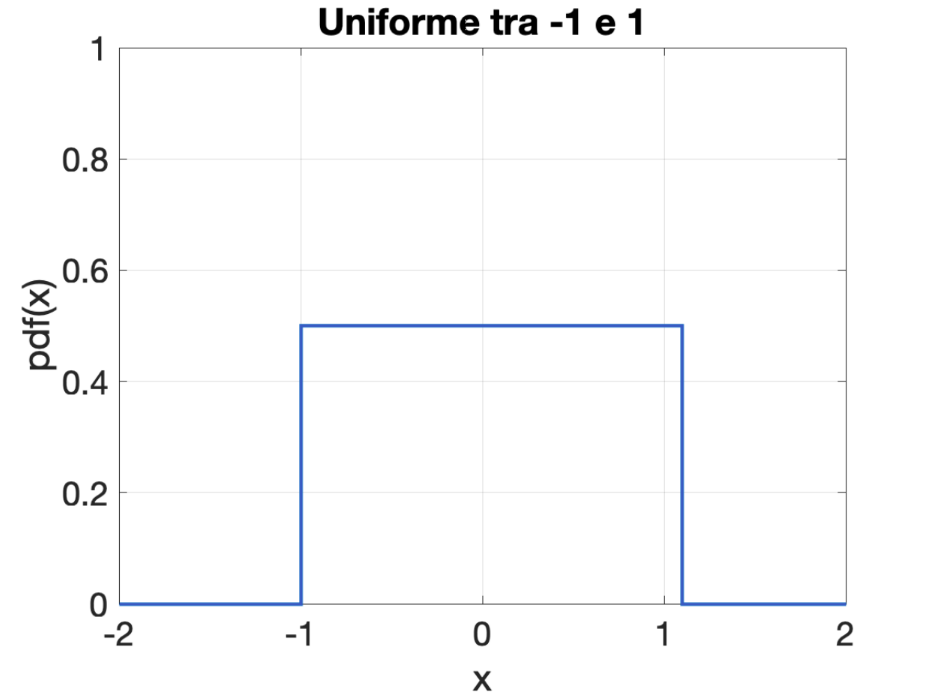
\includegraphics[width=5cm]{uniforme-pdf} \caption{}
			\end{subfigure}
			\begin{subfigure}{0.48\linewidth}
				\centering
				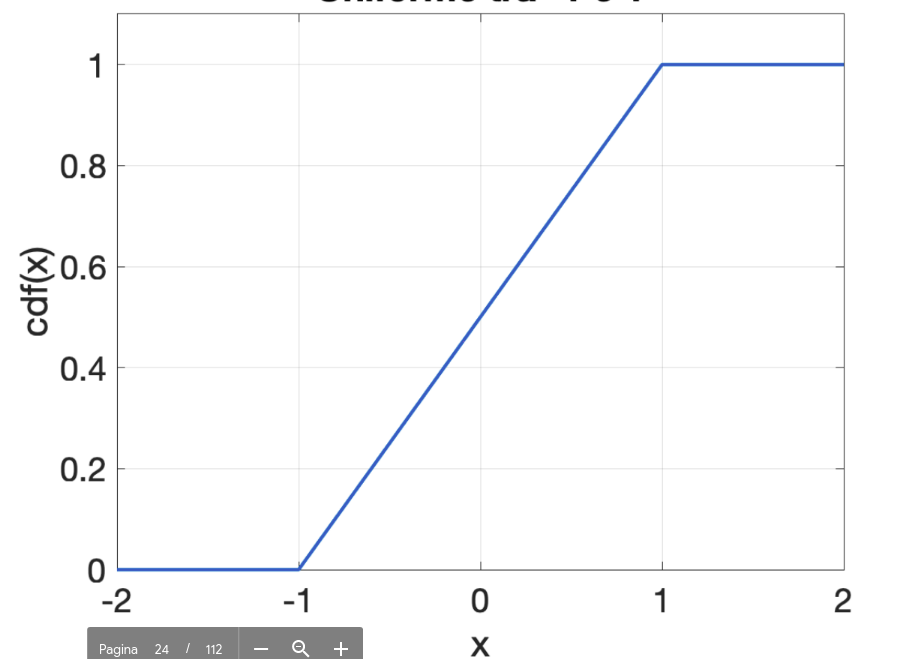
\includegraphics[width=5cm]{uniforme-cdf} \caption{}
			\end{subfigure}
			\caption{funzione PDF (a) e CDF (b) di una distribuzione uniforme $U(-1,1)$.}
			\label{fig:stat:uniforme}
		\end{figure}
		
		\paragraph{Distribuzione normale o gaussiana} Un evento statistico $y$ si comporta come \de{distribuzione normale} (o \de{gaussiana}) $y \backsim N(\mu , \sigma^2)$ di media $\mu$ e varianza $\sigma^2$ (figura \ref{fig:stat:gaussiana}) se al sua PDF segue una relazione del tipo
		\begin{equation}
			f_{pd}(y) = \frac 1 {\sigma \sqrt{2\pi}} e^{-\dfrac 1 2 \left[\dfrac{y-\mu}{\sigma}\right]^2}
		\end{equation}
		
		Una generica distribuzione gaussiana di valore atteso $\mu$ e varianza $\sigma^2$ può essere normalizzata per diventare una distribuzione normale di valore atteso $0$ e varianza unitaria secondo la legge
		\begin{equation}
			\frac{y -\mu}{\sigma} \backsim N(0,1)
		\end{equation}
		Caratteristica della distribuzione gaussiana normalizzata è che la probabilità di ottenere un valore stocastico $x$ nell'intervallo $(-3,3)$ è pari al $99.7\%$.
		
		
		\begin{figure}[bht]
			\centering
			\begin{subfigure}{0.48\linewidth}
				\centering
				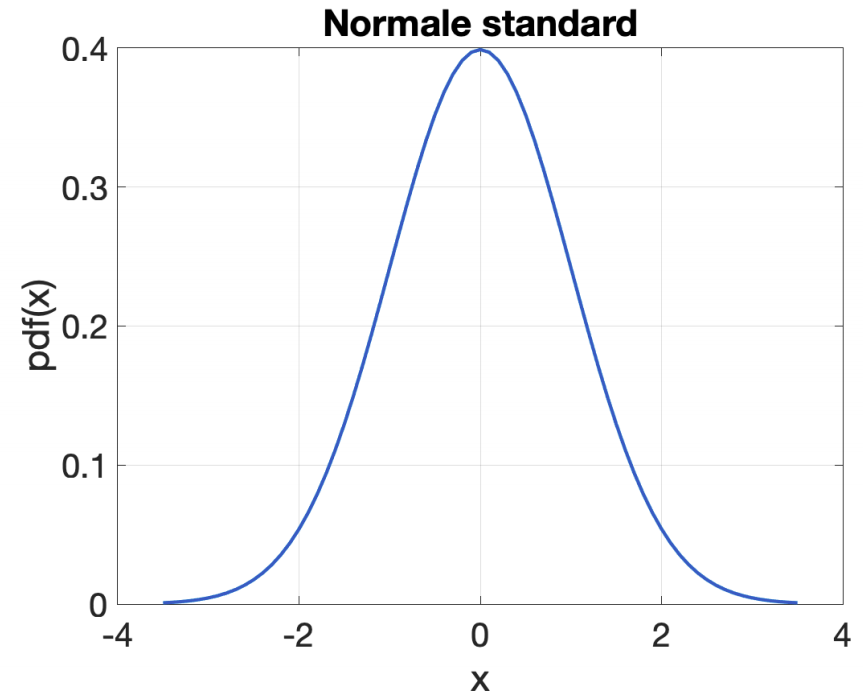
\includegraphics[width=5cm]{gaussiana-pdf} \caption{}
			\end{subfigure}
			\begin{subfigure}{0.48\linewidth}
				\centering
				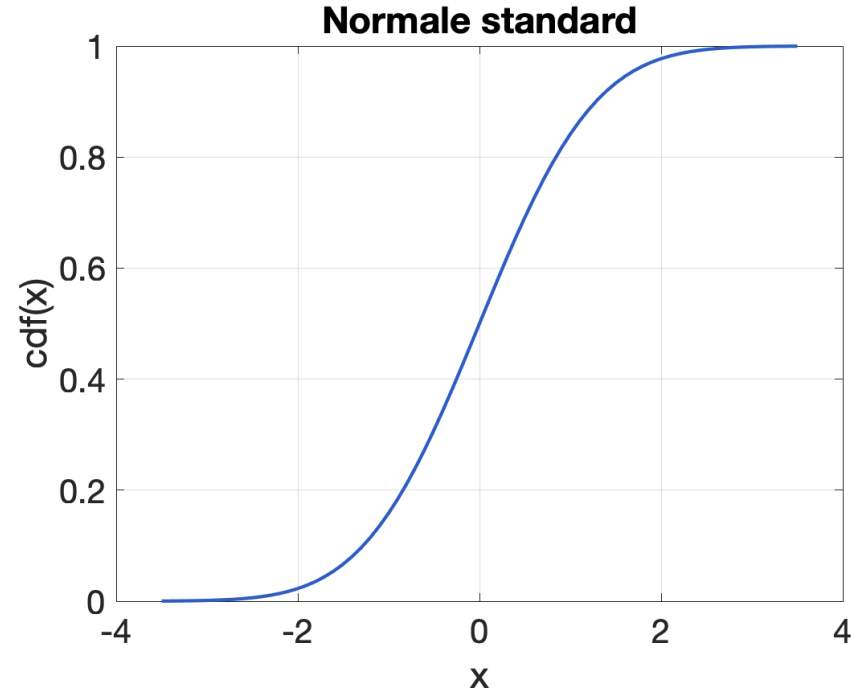
\includegraphics[width=5cm]{gaussiana-cdf} \caption{}
			\end{subfigure}
			\caption{funzione PDF (a) e CDF (b) di una distribuzione gaussiana standard $N(0,1)$.}
			\label{fig:stat:gaussiana}
		\end{figure}
		
		\paragraph{Distribuzione chi-quadro} Un variabile stocastica $y$ è approssimata ad una \de{distribuzione xhi-quadro} $\chi^2_k$ di ordine $k$ (figura \ref{fig:stat:chiquadro}) se può essere scritta come una somma di distribuzioni normali al quadrato:
		\begin{equation}
			y \backsim \chi_k^2 \qquad \Leftrightarrow \qquad y = z_1^2 + z_2^2 + \dots + z_k^2 \quad \textrm{con } z_i\backsim N(0,1)
		\end{equation}
		La funzione PDF $f_{pd}(y)$ può essere calcolato utilizzando la funzione gamma $\Gamma$ di Eulero ed è determinata come
		\begin{equation}
			f_{pd}(y) = \frac 1 {2^{k/2} \, \Gamma \big(k/2\big) } y ^{\frac k 2 - 1} e^{-\frac y 2}
		\end{equation}
		Di questa distribuzione è possibile osservare che il valore atteso $\mu$ coincide con l'ordine della funzione, ossia $\mu = k$; la varianza della stessa risulta essere invece $\sigma^2 = 2k$.
		
		Definendo con $ss$ la somma degli scarti quadratici medi di un campione di media $\ov y$, allora il suo rapporto con lo scarto quadratico medio $\sigma^2$ della relativa popolazione si distribuisce come una chi-quadro secondo la relaizone
		\begin{equation}
			\frac{ss}{\sigma^2} = \frac{\sum_{i=1}^2 \big(y_i-\ov y\big)^2}{\sigma^2} \backsim \chi_{n-1}^2
		\end{equation}
		
		\begin{figure}[bht]
			\centering
			\begin{subfigure}{0.48\linewidth}
				\centering
				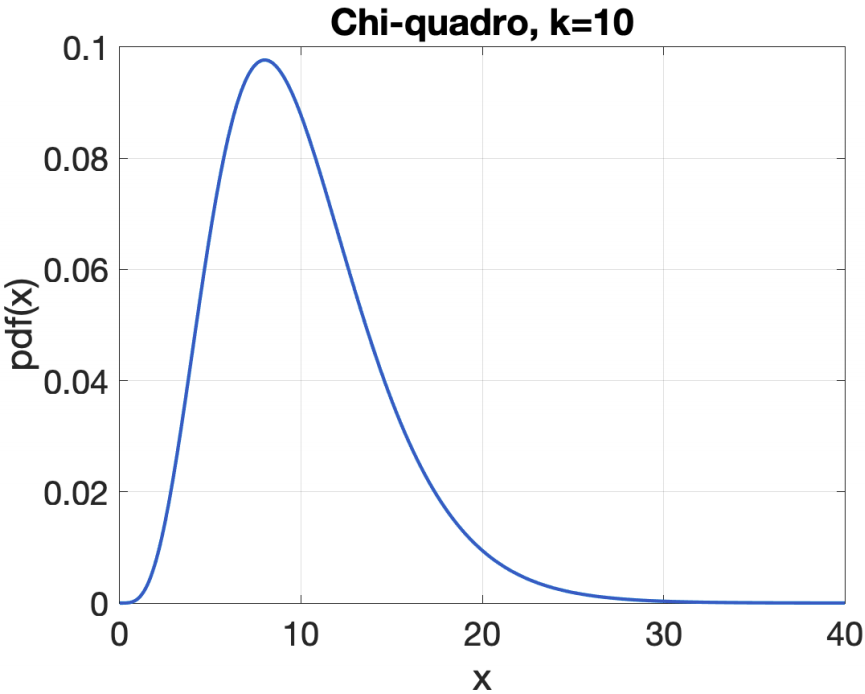
\includegraphics[width=5cm]{chiquadro-pdf} \caption{}
			\end{subfigure}
			\begin{subfigure}{0.48\linewidth}
				\centering
				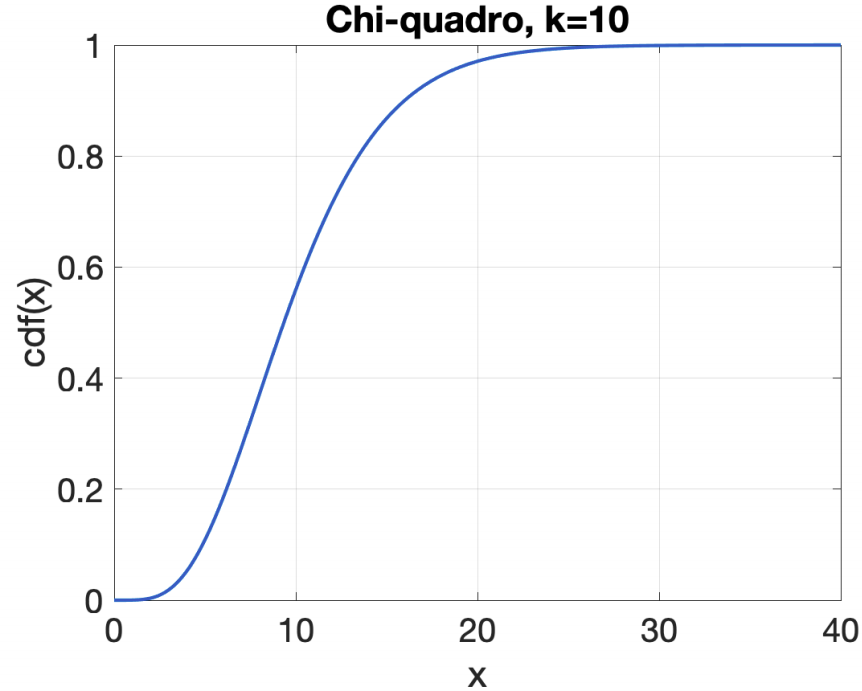
\includegraphics[width=5cm]{chiquadro-cdf} \caption{}
			\end{subfigure}
			\caption{funzione PDF (a) e CDF (b) di una distribuzione chi-quadro $\chi^2_{10}$ di ordine $k=10$.}
			\label{fig:stat:chiquadro}
		\end{figure}
		
		\paragraph{Distribuzione T di Student} Una variabile stocastica $y$ è \de{distribuita} come una \de{T di Student} $y \backsim t_k$ di ordine $k$ se è esprimibile nella forma
		\begin{equation}
			y \backsim t_k \qquad \Leftrightarrow \qquad y = \frac z {\sqrt{x/k}} \quad \textrm{con } z \backsim N (0,1) \ , \ x \backsim \chi_k^2
		\end{equation}
		La relativa PDF può essere espressa come
		\begin{equation}
			f_{pd}(y) = \frac{\Gamma \left(\frac{k-1}{2}\right)}{\sqrt{k\pi} \, \Gamma \left( \frac k 2 \right)} \frac 1 {\left(\frac{y^2}{k} + 1 \right)^{(k+1)/2}}
		\end{equation}
		Questa funzione è caratterizzata dall'avere valore atteso $\mu = 0$ e varianza $\sigma^2 = \frac{k}{k+2}$. E' possibile osservare che per $k\rightarrow \infty$ la distribuzione T di Student tende ad assumere una distribuzione normale (l'approssimazione è valida in generale per $k>50$):
		\[ t_k \quad \xrightarrow{k\rightarrow \infty} \quad N(0,1)\]
		
		\begin{figure}[bht]
			\centering
			\begin{subfigure}{0.48\linewidth}
				\centering
				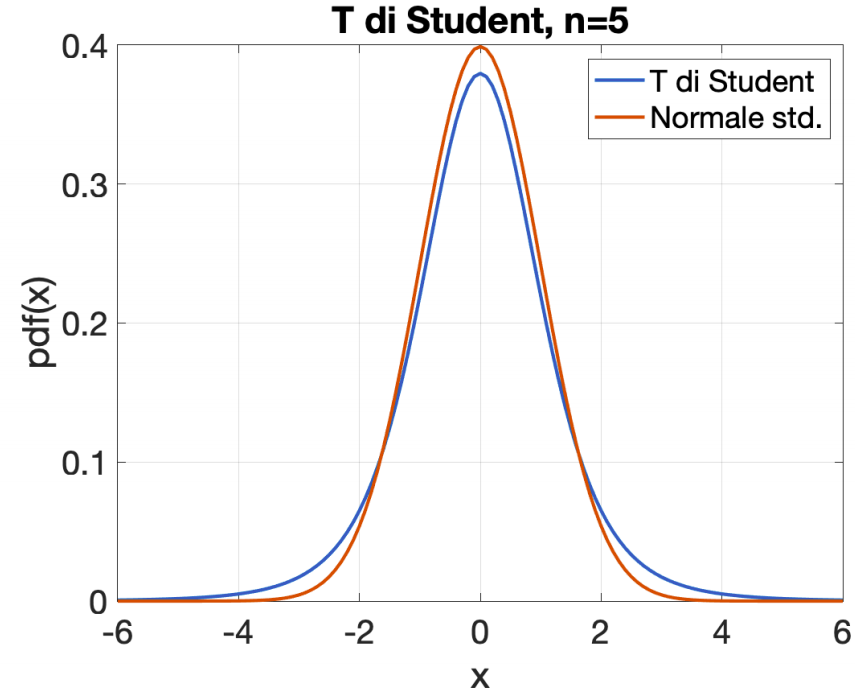
\includegraphics[width=5cm]{student-pdf} \caption{}
			\end{subfigure}
			\begin{subfigure}{0.48\linewidth}
				\centering
				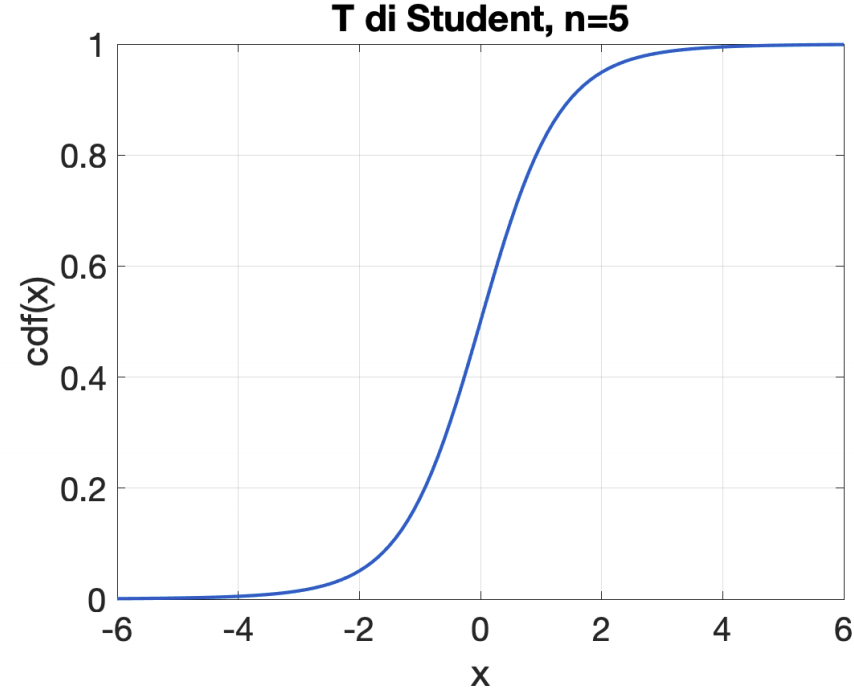
\includegraphics[width=5cm]{student-cdf} \caption{}
			\end{subfigure}
			\caption{funzione PDF (a), in relazione ad una normale, e CDF (b) di una distribuzione T di Student $t_5$ di ordine $k=5$.}
			\label{fig:stat:student}
		\end{figure}
		
		
	\subsection{Distribuzione della media e teorema del limite centrale}
		
		\paragraph{Distribuzione della media} Si consideri $x_i \backsim N(\mu, \sigma^2)$, ossia una variabile aleatoria  con distribuzione normale di valore atteso $\mu$ e varianza $\sigma_2$. E' possibile verificare che la \de{media campionaria} $\ov x$ di un campione assume una distribuzione normale in quanto somma delle stesse:
		\begin{align*}
			E\big(\ov x\big) & = E \left(\frac{x_1 + x_2 + \dots  
			 + x_n}{n}\right) = \frac 1 n \, E\left(x_1 + x_2+\dots +x_n\right) \\ 
		 	& = \frac 1 n \Big[ E(x_1) + E(x_2) + \dots + E(x_n)\Big] = \frac 1 n n E(x) \\
		 	& = \mu 
		\end{align*}
		
		A questo punto è possibile stabilire, tramite l'operatore varianza, la varianza $s_{\ov x}^2$ del campione di variabili $x$ (ognuna delle quali di varianza $s_x^2$) utilizzando le relazioni
		\begin{align*}
			V\big(\ov x\big) & = V \left( \frac{x_1 + x_2 + \dots + x_n}{n} \right) = \left(\frac 1 n\right)^2 \, V\big(x_1+x_2+\dots +x_n\big) \\
			& = \frac 1 {n^2} \Big[ V(x_1) + V(x_2) + \dots + V(x_n) \Big] = \frac n {n^2} V(x) = \frac 1 n V(x) \\
			& = \frac{s_x^2}{n}
		\end{align*}	
		A questo punto è possibile osservare che la distribuzione di una media campionaria di valori di distribuzioni normali è anch'essa una gaussiana di valore atteso $\mu$ ma varianza $\sigma^2/n$ e dunque
		\[ \ov x \backsim N\big(\mu , \sigma^2/n\big) \]	
		
		\subsubsection{Teorema del limite centrale}
		\paragraph{Enunciato} {\itshape Se $x_1,x_2,\dots, x_n$ sono $n$ variabili aleatorie indipendenti ed egualmente distribuite con valore atteso $E(x_i)=\mu$ e varianza $V(x_i) = \sigma^2$ (entrambi valori finiti), e si consideri $y = x_1+x_2+\dots + x_n$, allora
		\[ z_n = \frac{y - n\mu }{\sqrt{n\sigma^2}} \]
		è distribuita approssimativamente come una gaussiana $N(0,1)$ nel senso che, se $F_n(z)$ è la densità di probabilità di $z_n$ e $\Phi(z)$ è la PDF di una variabile casusale di tipo $N(0,1)$, allora
		\[\lim_{n\rightarrow \infty} \frac{F_n(z)}{\phi(z)} = 1\] }
		
		\paragraph{Osservazioni} Da questo teorema deriva il fatto che la distribuzione gaussiana è detta normale in quanto occupa un posto centrale per il limite a cui tendono le distribuzioni delle somme. Questo è un teorema molto robusto rispetto alle ipotesi: ogni  misurazione dipende da numeri fattori casuali (dovuti al misurando, ai trasduttori, ai rumori ambientali e dell'operatore..) che determina con elevata probabilità che la componente casuale dei valori sia distribuita in maniera normale.
		
\section{Statistica inferenziale}
	La \de{statistica inferenziale} è il procedimento per cui si inducono le caratteristiche di una popolazione dall'\textbf{osservazione di un campione estratto a caso} della stessa. 
	
	Una parte fondamentale della statistica inferenziale sono i \de{test statistici}, ossia dei particolari tesi in cui ci si domanda se un dato campione sia o meno compatibile con la rispettiva popolazione di riferimento (valutandone il valore atteso, la varianza e la distribuzione). \\
	In particolare un test statistico serve a decidere quale di due \textbf{ipotesi opposte} ha più probabilità di essere errata; si definiscono dunque l'\de{ipotesi nulla} $H_0$ quella debole (che tipicamente corrisponde ad un'osservazione non significativa) e l'\de{ipotesi alternativa} $H_1$ come la scelta forte, diversa dal valore atteso. In linea di principio dato un campione di media campionaria $\ov x$ e valore atteso della popolazione $\mu_0$ le due ipotesi sono caratterizzate dall'espressione
	\[ H_0:\ \ov x \simeq  \mu_0 \qquad H_1:\ \ov x \neq \mu_0 \]
	
	\begin{esempio}{: ipotesi in un impianto industriale} \label{es:stat:impianto}
		Considerando di vole effettuare un test statistico su un impianto industriale (per esempio verificare che i diametri dei tubi siano coerenti rispetto al valore richiesto) allora:
		\begin{itemize}
			\item l'ipotesi nulla $H_0$, quella debole, è associata al corretto funzionamento dell'impianto in quanto la distribuzione dei campioni analizzati è in linea con la distribuzione teorica della fabbrica;
			\item l'ipotesi alternativa $H_1$, quella forte, è associata ad uno scorretto funzionamento dell'impianto che produce tubi con diametri statisticamente incompatibili con il valore nominale.
		\end{itemize}
	\end{esempio}
	
	Le ipotesi si raggruppano tipicamente nella cosiddetta \de{matrice di confusione} che correla la verità dell'ipotesi nulla $H_0$ con la decisione presa di accettarla o rifiutarla:
	\begin{SCtable}[0.5][h!]
		
		\begin{tabular}{ c | c c}
			$H_0$ &  vera & falsa \\ \hline \hline 
			accettata & ok & {$\beta$: errore di tipo II  } \\
			rifiutata & $\alpha$: errore di tipo I  & ok
		\end{tabular}
		
		\caption{matrice di confusione.}
	\end{SCtable}
	
	Si può osservare che accettando l'ipotesi nulla quando essa è verifica (e analogamente rifiutarla quando essa è falsa) comporta una scelta corretta del comportamento da seguire
	
	L'\de{errore di tipo I} può essere considerato come un \textbf{falso allarme} e si verifica quando si rifiuta un'ipotesi nulla vera; questo tipo di errore è valutato dal parametro $\alpha$.	Accettando invece l'ipotesi falsa si ha un \de{errore di tipo II}, ossia un \textbf{mancato allarme}, ed è valutato dalla probabilità $\beta$; il termine $1-\beta$ rappresenta dunque la \de{potenza} del test statistico. I valori $\alpha$ e $\beta$ non sono necessariamente correlati.
	
	\begin{esempio}{: matrice di confusione in un impianto industriale}
		Facendo riferimento all'esempio \ref{es:stat:impianto}, è possibile associare la matrice di confusione ai seguenti stati di funzionamento con l'obiettivo di fermare l'impianto nel caso in cui esso produca pezzi non congruenti all'obiettivo.
		
		Nel caso in cui l'ipotesi nulla $H_0$ sia verificata allora l'impianto sta producendo correttamente i pezzi:
		\begin{itemize}
			\item accettando l'ipotesi l'impianto continuerà a produrre ed è una scelta corretta, in quanto non ci sono problemi di funzionamento del sistema;
			\item rifiutando questa ipotesi allora si considera che il sistema stia producendo pezzi difettosi quando la realtà è diversa: si ha dunque un falso allarme in quanto l'impianto si fermerebbe nonostante dovrebbe continuare a produrre.
		\end{itemize}
	
		Nel caso in cui l'ipotesi nulla $H_0$ sia falsa allora l'impianto sta producendo pezzi non conformi all'obiettivo:
		\begin{itemize}
			\item rifiutando l'ipotesi l'impianto si ferma  in quanto è riuscito ad individuare correttamente il suo malfunzionamento;
			\item accettando invece l'ipotesi nulla allora l'impianto, nonostante stia sbagliando, pensa di produrre i pezzi in maniera corretta ed è per questo che si parla di mancato allarme: l'impianto non rileva uno stato di funzionamento erroneo.
		\end{itemize}
	\end{esempio}

	\subsection{Analisi di un campione}  \label{sec:stat:teststudent}
		\paragraph{Test di Student} Considerando un campione di $n$ valori aleatori $x_i$ è possibile standardizzare la media campionaria $\ov x$ sottraendo alla stessa il valore atteso $\mu_0$ del test e dividendo il tutto per la deviazione standard del campione (divisione $s/\sqrt n$) ottenendo il risultato
		\[ t_0 = \frac{\big|\ov x- \mu_0\big|}{s/\sqrt n} \backsim t_n \]
		Si osserva dunque che il risultato normalizzato è distribuito come una t di student con parametro $n$ pari al numero di campioni. Il risultato $t_0$ è detto dunque \de{statistica di test}.
		
		Intuitivamente la statistica $t_0$ è tanto più grande quanto più la media campionaria è distante dal valore atteso relativamente alla sua varianza. Tanto più è piccola la probabilità di riscontrare un valore maggiore di $t_0$ sulla distribuzione T di Student, tanto più possiamo dedirre che il campione con media $\ov x$ e varianza $s^2$ \textbf{non proviene} da una popolazione con valore atteso $\mu_0$. La probabilità di riscontrare un valore maggiore di $t_0$ è dunque detto \de{\textit{p-}value} e rappresenta la probabilità di errore di tipo I $\alpha$.
		
		\begin{esempio}{: \textit{p-}value}
			Considerando un campione di $n=5$ elementi con media campionaria $\ov x$ e varianza $s^2$ tali da generare una statistica di test $t_0=2$:
			\[ t_0 = \frac{|\ov x - \mu_0|}{s/\sqrt 5} = 2 \]
			Determinata la funzione CDF lower tail $f_{cd,l}(t)$ associata alla distribuzione T di Student di parametro 5, allora è possibile determinare il $\pval$ di questa statistica come
			\[ \pval = 2\Big[1- \, f_{cd,l}(t_0) \Big] = 2\, f_{cd,u}(t_0) = 0.046 \]
			Questo significa che la probabilità di errore di affermare che la differenza tra $\ov x$ e $\mu_0$ è significativa è pari al $4.6\%$.
			
			\vspace{3mm}
			Si osserva che nell'espressione del $\pval$ si ha la moltiplicazione per un fattore 2 dovuta al fatto che la distribuzione T di Student è simmetrica ed è necessario considerare anche il rispettivo valore negativo di $t_0$.
		\end{esempio}
		
		Ipotizzando di conoscere la varianza $\sigma^2$ della popolazione della quale si estrae il campione, allora la statistica di test risutla distribuita come una normale standard e assume la forma
		\[ z_0 = \frac{|\ov x - \mu_0|}{\sigma/\sqrt n} \backsim N(0,1) \]
		In generale più $n$ è grande più la distribuzione $t_k$ T di Student di ordine $k$ assomiglia ad una normale standard $N(0,1)$; in generale per un numero di campioni $n>50$ è possibile effettuare l'approssimazione di $t_0$ alla rispettiva distribuzione normale: $t_0\approx z_0$.
		
		
	\subsection{Analisi di normalità}
		L'\de{analisi di normalità} serve per verificare se un campione è più o meno compatibile con una distribuzione normale ed è basata su due tipi di analisi:
		\begin{itemize}
			\item \textbf{analisi dei quantili} del campione e relativo confronto con i quantili di una distribuzione normale; questo è un approccio grafico e dunque soggettivo;
			\item \textbf{analisi} basata su \textbf{test statistici} dove si considera come ipotesi nulla $H_0$ che la distribuzione analizzata sia normale; questo è un approccio oggettivo.
		\end{itemize}
		
		\subsubsection{Analisi dei quantili}
		Il \de{quantile} può essere considerato come la funzione inversa della cumulata di una distribuzione.
		
		
		
		\subsubsection{Test del chi-quadro} 
		Un test statistico per determinare la normalità (o meno) di una distribuzione campionaria può essere effettuato tramite il cosiddetto \de{test del chi-quadro}. 
		
		Essendo questo un test statistico si considera come \textbf{ipotesi nulla} $H_0$ quella che afferma che il campione è distribuito normalmente, mentre l'\textbf{ipotesi alternativa} $H_1$ è quella riferita alla non normalità di distribuzione del campione.
		
		Per effettuare il test è necessario dividere gli $n$ campioni da analizzare in $k$ classi di 4-5 valori l'una. Definendo $O_i$ il numero di osservazioni nell'$i-$esima classe, ad ognuna di esse sarà associato un valore atteso $E_i$ rispetto ad una distribuzione normale che può essere determinata tramite la sua CDF come
		\[ E_i = f_{cd,l}\big(\textrm{max}_k \big) - f_{cd,l}\big(\textrm{min}_k\big)\]
		A questo punto è possibile determinare la \de{statistica di test} $X_0^2$ per il test statistico in questione come
		\[ X_0^2 = \sum_{i=1}^k \frac{\big(O_i - E_i\big)^2}{E_i} \backsim 	\chi^2_{k-p-1}  \]
		
		La statistica di test è una somma di quadrati di variabili casuali ed approssima dunque la distribuzione chi-quadro come indicata; questa approssimazione è tanto più fedele quanto maggiore è il numero di campioni analizzati. Il parametro della distribuzione $\chi^2$ è il numero di elementi indipendenti nella somma che coincide al valore $k-1-p$, dove $k$ è il numero di classi individuate e $p$ è il numero di parametri della distribuzione di riferimento (2 per la distribuzione normale: $\mu$ e $\sigma^2$).
		
		Come nel caso del test T di Student, il $\pval$ del test statistico in questione è determinato dalla probabilità di trovare il valore $X_0^2$ nella distribuzione $\chi^2$; non essendo questo test simmetrico il $\pval$ è determinato tramite la CDL della distribuzione chi-quadro come
		\[\pval = \min \Big\{f_{cd,l}\big(X_0^2\big), f_{cd,u}\big(X_0^2\big)\Big\}\]
		Il $\pval$ rappresenta dunque l'errore nel rigettare l'ipotesi nulla, ossia l'errore che si commetterebbe a considerare la distribuzione di partenza come non normale.
		
		\begin{nota}
			Il test del chi-quadro può essere effettuato non solo per verificare la normalità di una distribuzione, ma per effettuare un confronto tra qualsiasi distribuzione: per fare questo è sufficiente sostituire al criterio di normalità $E_i$ la relazione del valore atteso della distribuzione di riferimento.
		\end{nota}
		
		\subsubsection{Test di contingenza}
		In certi casi $n$ elementi di una popolazione possono essere \textbf{classificati} secondo \textbf{due criteri differenti}: in tal caso è interessante sapere se i due criteri di classificazione siano \textbf{statisticamente indipendenti} o meno.
		
		A questo punto i dati osservati $O_{ij}$ possono essere raggruppati nella cosiddetta \de{tabella di contingenza} che riporta nelle righe il numero di osservazioni che ricadono nel primo criterio, nelle colonne quelle del secondo criterio.
		
		Per effettuare un test di contingenza si consideri il caso di voler sapere se 3 piani di assicurazioni distinti sono preferiti da impiegati salariati o a cottimo basandoci sulla seguente tabella di contingenza:
		\begin{center}
		\begin{tabular}{ c || p{1.5cm} p{1.5cm} p{1.5cm} | c}
			& \multicolumn{3}{c |}{piano assicurativo} & \\
			impiego & \centering piano 1 & \centering piano 2 & \centering piano 3 & totale \\ \hline \hline
			salariato & \centering 160 & \centering 140 & \centering 40 & 340 \\
			a cottimo & \centering 40 & \centering 60 & \centering 60 & 160 \\ \hline 
			totale & \centering 200 & \centering 200 & \centering 100 & 500
		\end{tabular}
		\end{center}
	
		Della tabella è necessario determinare i totali cumulativi sia per riga che per colonna; dividendo questi valori per le osservazioni totali si determinano i \de{totali marginali} $\hat u_i$ (della riga $i-$esima) e $\hat v_j$ (per la colonna $j-$esima); in particolare definendo con $r$ il numero di righe e $c$ il numero di colonne, allora i totali marginali in maniera esplicita sono determinati come
		\[ \hat u_i = \frac 1 n \sum_{j=1}^c O_{ij} \qquad \hat v_j = \frac 1 n \sum_{i=1}^r O_{ij} \]
		Rispetto alla tabella di contingenza in esempio è possibile affermare che i totali marginali per riga valgono $\hat u_1 = 340/500 = 0.68, \hat u_2 = 160/500 = 0.32$, mentre per le colonne $\hat v_1 = 200/500 = 0.4, \hat v_2 = 0.4, \hat v_3 = 0.2$.
		
		Questi totali marginali sono due criteri indipendenti e rappresentano i valori attesi di ciascun criterio: possono dunque essere utilizzati per calcolare i valori attesi $E_{ij}$ di ogni combinazione di criteri:
		\[ E_{ij} = n \hat u_i \hat v_j = \frac 1 n \sum_{j=1}^c O_{ij} \, \sum_{i=1}^r O_{ij} \]
		
		A questo punto è possibile effettuare un \textbf{test chi-quadro} considerando come espressione del valore atteso quella appena descritta, e in particolare si determina la \de{statistica di test} $X_0$ da confrontare con la distribuzione $\chi^2$:
		\[X_0^2 = \sum_{j=1}^c \sum_{i=1}^r \frac{\big(O_{ij} - E_{ij} \big)^2}{E_{ijx}}\]
		
		Il $\pval$ associata alla distribuzione rappresenta l'errore statistico nel considerare i due eventi come dipendenti.
		
	\subsection{Anomalie}
		Un'\de{anomalia} (\textit{outlier}) è un'osservazione non compatibile con la distribuzione del resto del campione; essa più risultare da un errore nella conduzione della misura o nella trascrizione/registrazione del valore misurato stesso.
		
		Questo è un \textbf{evento raro} associato ad una distribuzione differente da quella tipica del processo di misura correttamente eseguito; in generale ci si attende non più di un'anomalia per campione (altrimenti si potrebbe pensare che i valori siano dovuti ad una somma di distribuzioni) e devono dunque essere eliminate per ridurre la varianza della distribuzione rispetto al valore atteso. Le anomalie hanno chiaramente effetti più forti su campioni piccoli.
		
		Per la rimozione delle anomalie è possibile utilizzare il \de{criterio di Chauvenet} o il \de{test di Grubb}, con l'accortezza di non applicare ciascun criterio più di una volta.
		
		\paragraph{Criterio di Chauvenet} Data una serie di $n$ osservazioni $x_i$ che generano una media campionaria $\ov x$ e deviazione standard $s_x$, allora è possibile calcolare lo scarto massimo assoluto $s_0$ come
		\[ s_0 = \max_{i=1,\dots, n} \left(\frac{|x_i - \ov x|}{s_x}\right)  \] 
		
		A questo punti si calcola la probabilità $P_s$ di avere un valore maggiore di $s_0$ sulla normale standard usando le funzioni PDF e CDF della stessa, e dunque:
		\[P_s =P\big(x>s_0\big) = \int_{s_0}^{+\infty} f_{pd}(\xi)\, d\xi = 1 - f_{cd,l}\big(s_0\big) = f_{cd,u}\big(s_0\big)  \]
		
		Su $n$ osservazioni, il numero di elementi attesi con scarto maggiore di $s_0$ è pari ad $n\, P_s$; se tale valore è inferiore a $n\, P_s < 0.5$ allora si elimina il dato con lo scarto maggiore assoluto.
		\begin{nota}
			La procedura non può essere ripetuta più di una volta in quanto porta ad un'alterazione della distribuzione.
		\end{nota}
	
		\paragraph{Test di Grubb} Il \de{test di Grubb} è un metodo statistico per eliminare le anomalie; analogamente date $n$ osservazioni $x_i$ si determina lo scarto massimo assoluto $s_0$ dipendente dalla media campionaria $\ov x$ e la relativa deviazione standard $s_x$. A questo punto si deve verificare se
		\[ s_0 > \frac{ n - 1}{n} \sqrt{\frac{t^2_{\alpha/(2n), n-2}}{n-2+t^2_{\alpha/(2n), n-2}}} \]
		dove $t_{\alpha,k}$ è il quantile $\alpha$ della distribuzione T di Student con parametro $k$.
		
		Se la disuguaglianza risulta essere verificata allora si elimina l'osservazione associata allo scarto massimo $s_0$.
		
\section{Analisi di regressione}		
	L'\de{analisi di regressione} è una serie di strumenti matematici che servono ad identificare i parametri di una legge, ossia un \textbf{modello matematico}, che meglio adattano la stessa a delle osservazioni.
	
	In particolare il \de{modello} è una funzione $f$ che determina la \de{risposta} $y$ in relazione al \de{predittore} $x$ secondo l'espressione $y = f(x)$.
	
	\figura{5}{1}{regressione}{dati campionari (puntini) e relativa funzione di regressione (linea rossa continua).}{esregr}
	
	Considerando l'esempio in figura \ref{esregr}, è possibile osservare che i campioni sembrano disporsi secondo una legge quadratica, seguendo dunque un modello $f(x)$ del tipo:
	\[ y = ax^2+bx+c \]
	Effettuare l'analisi di regressione significa dunque determinare i coefficienti $a,b,c$ che meglio adattano il modello ai dati campionari raccolti.
	
	Il modello di partenza del quale fare la regressione può essere sia semplice (come una retta), sia molto complicato (funzioni non lineari implicite), sia monodimensionale che multidimensionale; il \textbf{numero di dimensioni} $n$ di un modello è il numero di predittori $x_1, \dots, x_n$ utilizzati per effettuare la regressione stessa.
	
	Il \de{modello} può essere sia \de{lineare} che \de{non lineare}, e la catalogazione deve essere effettuata osservando i coefficienti, come nell'esempio seguente:
	\[ \textrm{lineare: } y = c_0 +c_1x_1^2+c_2x_1^2+c_3x_2+c_4x_1x_2 \qquad \textrm{non lineare: } y = \frac{c_1x_1 \cos\big(c_2x_2\big)}{c_3x_3}\]
		
	\paragraph{Regressione ai minimi quadrati} In generale per effettuare questo tipo di analisi, ossia determinare i coefficienti che meglio adattano il modello ai campioni, si utilizza la \de{regressione ai minimi quadrati} che adotta come \de{indice di prestazione} $\Phi$ lo scarto quadratico medio sui punti campionati $\big\langle x_1, \dots, x_N\big\rangle$:
	\begin{equation}
		\Phi\big(c_1, \dots, c_n\big) = \sum_{i=1}^N \epsilon_i^2 \qquad \textrm{con} \quad \epsilon_i^2 = y_i- f\big(c_1, \dots, c_n, x_i\big)
	\end{equation}
	La soluzione del problema è dunque la minimizzazione dell'indice di prestazione $\Phi$.
	
	\begin{esempio}{: regressione lineare}
		Per effettuare una \textbf{regressione lineare}, ossia basata sul modello $y = ax + b$, è necessario considerare che la distanza tra modello e campione è data dall'espressione $\epsilon_i = y_i -\big(ax_i+b\big)$, e dunque il problema per essere risolto richiede la minimizzazione dell'indice di prestazione $\Phi$ dipendente solamente dai parametri $a$ e $b$, e dunque
		\[ \min_{a,b} \,\Phi(a,b) = \min_{a,b} \sum_{i=1}^N \Big[y_i - \big(ax_i+b\big)\Big]^2 \]
		Il minimo dell'espressione, che in questo caso è unico, si può trovare imponendo le derivate parziali di $\Phi$ nulle in funzione della posizione dei coefficienti $a,b$, ossia 
		\[ \frac \partial {\partial a} \Phi (a,b) = 0 \qquad  \frac \partial {\partial b} \Phi (a,b) = 0\]
		
		Svolgendo opportunamente i calcoli si dimostra che i valori ottimali dei coefficienti $a$ e $b$ valgono
		\[ a_\textrm{opt} = \frac{C_{xy}}{C_{xx}} \quad b_\textrm{opt} = \ov y - a\ov x \qquad \leftarrow  C_{xx} = \sum_{i=1}^N\big(x_i-\ov x\big)^2 \quad C_{xy} = \sum_{i=1}^N \big(x_i-\ov x\big)\big(y_i-\ov y\big) \]
		
		E' possibile inoltre determinare le varianze degli elementi fondamentali del modello che risultano valere
		\[ \sigma_y^2 = \frac{\sum_{i=1}^N \big[y_i-ax_i+b\big]^2}{N-2} \qquad \sigma_a^2 = \frac{\sigma_y^2}{C_{xx}} \qquad \sigma_b^2 = \sigma_y^2 \frac{\sum_{i=1}^N x_i^2}{N\, C_{xx}} \]
		
	\end{esempio}

	\subsection{Analisi di regressione di modelli lineari}
		Ogni modello di regressione di tipo lineare (nei coefficienti) può essere analizzato utilizzando una notazione matriciale; in particolare facendo riferimento ad un modello quadratico $ax^2 + bx + c$ (ma è possibile intuire che vale in generale per qualsiasi modello a coefficienti lineari) è possibile, date $N$ misurazioni $x_i$ e relativi risultati $y_i$, scrivere l'uscita vettoriale $\vett y$ come prodotto tra una matrice $\mathcal A\in \mathds{ R^{N\times n}}$ e il vettore dei coefficienti $\vett k$:
		\[ \begin{bmatrix}
			x_1^2 & x_1 & 1 \\
			x_2^2 & x_2 & 1 \\
			\vdots && \vdots \\
			x_N^2 & x_N & 1 
		\end{bmatrix} \begin{pmatrix}
			a \\ b \\ c
		\end{pmatrix} = \begin{pmatrix}
			y_1 \\ y_2 \\ \vdots \\ y_3 
		\end{pmatrix} \qquad \leftrightarrow \qquad \mathcal A \vett k = \vett y \]
		Per determinare il vettore dei coefficienti in maniera algebrica è dunque necessario utilizzare degli \textit{stratagemmi} matematici per rendere la matrice $\mathcal A$ quadrata e dunque invertibile, arrivando ai seguenti risultati:
		\begin{equation}
		\begin{split}
			\mathcal A^t \, \mathcal A \vett k & = \mathcal A^t \vett y \\
			\vett k & = \big(\mathcal A^t\mathcal A\big)^{-1} \mathcal A^t \vett y
		\end{split}
		\end{equation}
		
		Si osserva in generale che per effettuare un'analisi di regressione è necessario avere un numero di campioni che è superiore al numero dei coefficienti da determinare del modello.
		
	\subsection{Intervalli di predizione e confidenza} \label{sec:stat:regrpred}
		L'\de{intervallo di predizione} rappresenta la \textit{fascia} di entro la quale una futura osservazione possa ricadere entro una determinata probabilità, per esempio il $95\%$; in generale questo tipo di intervallo presenta un'ampiezza costante rispetto al modello determinato dalla regressione.
		
		L'\de{intervallo di confidenza} rappresenta invece l'intervallo in cui il modello atteso ha una probabilità di ricadere, ossia con quanta probabilità si ha la garanzia che il modello ottenuto dalla regressione sia fedele ai dati analizzati; questo tipo di intervallo non è in generale a sezione costante ma è particolarmente stretto nel \textit{centro} dei campioni analizzati, mentre tende ad \textit{allargarsi} nell'allontanarsi dal valor medio campionario.
		
		\figura{7}{1.2}{intervallipred}{regressione di un modello nominale (noto a priori) con relativi intervallo di predizione e confidenza (entrambi al $95\%$) rispetto ai campioni mostrati.}{intervallipred}
		
		A livello grafico, in linea generale, l'intervallo di predizione è più \textit{esterno} all'intervallo di confidenza, come si può osservare in figura \ref{intervallipred}.
		
	\subsection{Sovraadattamento e sottoadattamento}
		In generale una domanda lecita da porsi è quella di sapere se il campione è stato adattato \textit{bene} o meno dalla regressione: se il modello è appropriato ai dati, allora i residui\footnote{con \textit{residuo} si intende la distanza (con segno) tra il valore misurato $y_i$ del campione e quello che ci si aspetta dal modello $f(x_i)$.} sono casuali, privi di pattern e sono distribuiti normalmente (per via del teorema del limite centrale), e dunque è possibile confermare il risultato effettuando un testo di normalità come il chi-quadro. Un esempio di tale distribuzione è quella in figura \ref{fig:stat:sottoadattamento}.b.
		
		Si parla di \de{sottoadattamento} (\textit{underfitting}) quando è possibile osservare dei pattern nei residui e questo è dovuto alla \textit{poca curvatura} del modello utilizzato per la regressione dei dati, come si può osservare in figura \ref{fig:stat:sottoadattamento}.c.
		
		\begin{figure}[bht]
			\centering
			\begin{subfigure}{0.32\linewidth}
				\centering
				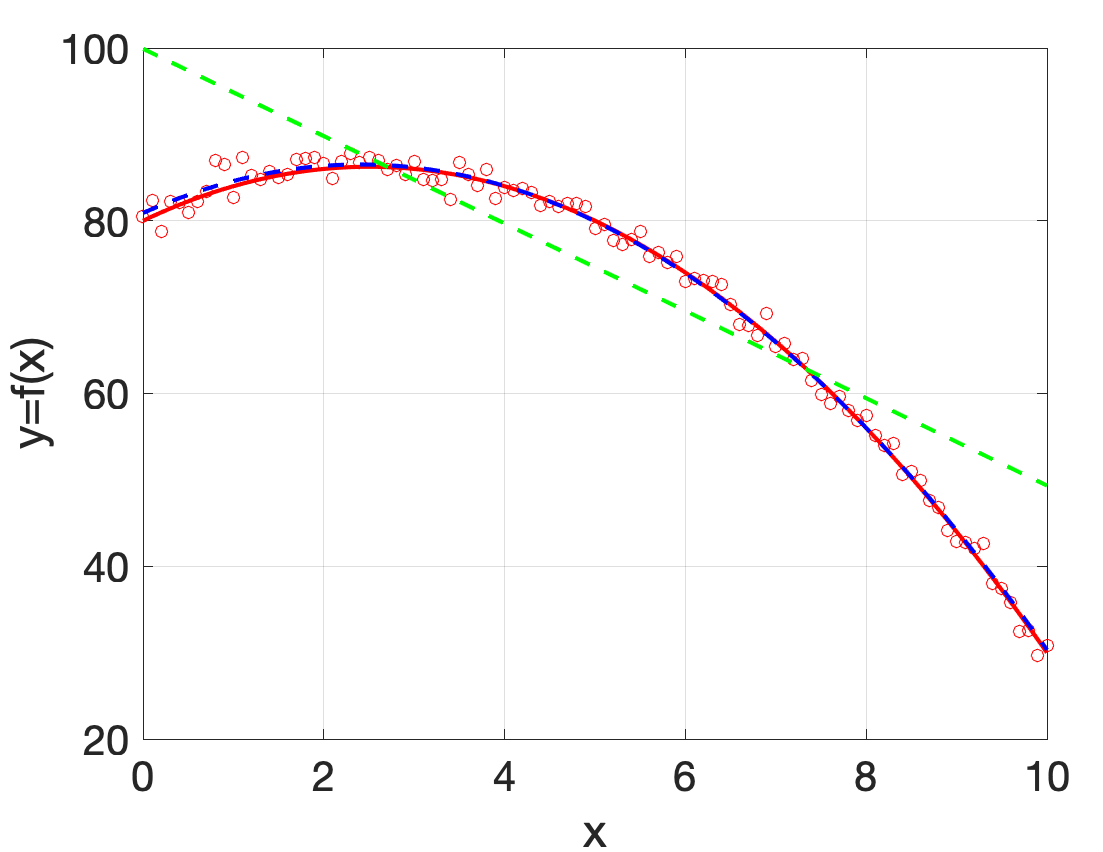
\includegraphics[width=0.9\linewidth]{sotto-a} \caption{}
			\end{subfigure}
			\begin{subfigure}{0.32\linewidth}
				\centering
				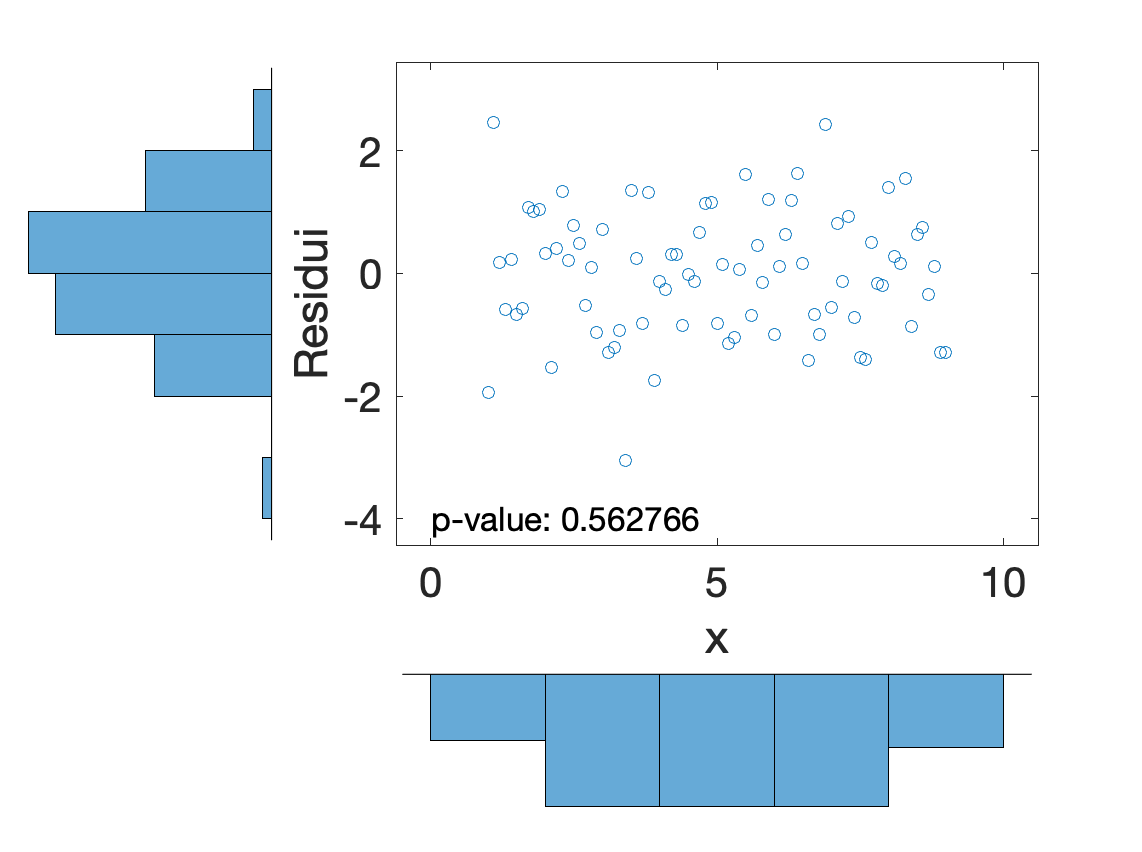
\includegraphics[width=0.9\linewidth]{sotto-b} \caption{}
			\end{subfigure}
			\begin{subfigure}{0.32\linewidth}
				\centering
				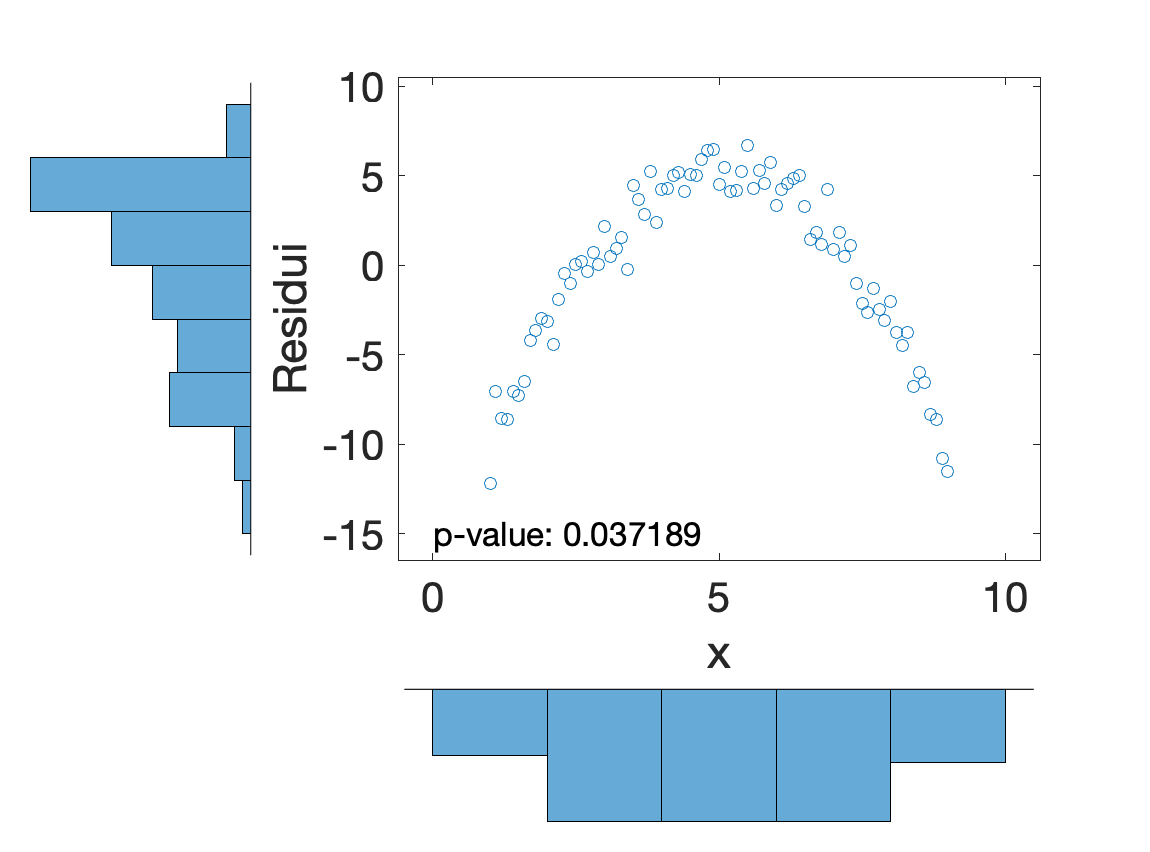
\includegraphics[width=0.9\linewidth]{sotto-c} \caption{}
			\end{subfigure}
			\caption{regressione lineare (in verde) e quadratica (in blu) di campioni distribuiti quadraticamente (curva nominale rossa) in figura $a$; in figura $b$ e $c$ sono mostrati rispettivamente i residui tra campioni e modello nel caso quadratico e lineare.}
			\label{fig:stat:sottoadattamento}
		\end{figure}
	
		Al contrario si parla di \de{sovraadattamento} (\textit{overfitting}) quando il modello utilizzato per effettuare la regressione è di ordine eccessivo al voluto; questo può essere notato considerando che al di fuori dell'\textit{intervallo di addestramento} (rappresentato dalle linee verticali tratteggiate in figura \ref{fig:stat:sovraadattamento}) il modello tende a divergere molto dai valori campionari esterni, e inoltre all'interno di questo range la funzione \textit{oscilla} per inseguire meglio i dati campionari.
		
		\begin{figure}[bht]
			\centering
			\begin{subfigure}{0.49\linewidth}
				\centering
				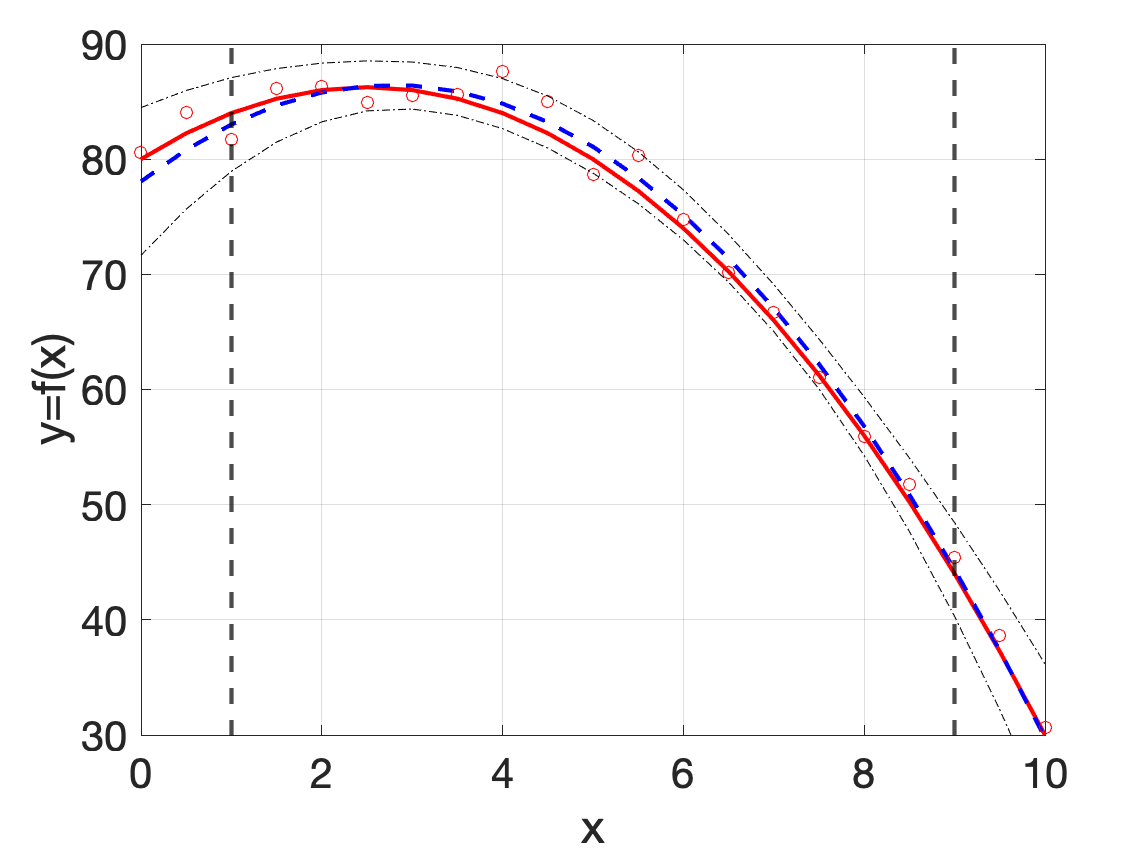
\includegraphics[width=0.7\linewidth]{sovra-a} \caption{}
			\end{subfigure}
			\begin{subfigure}{0.49\linewidth}
				\centering
				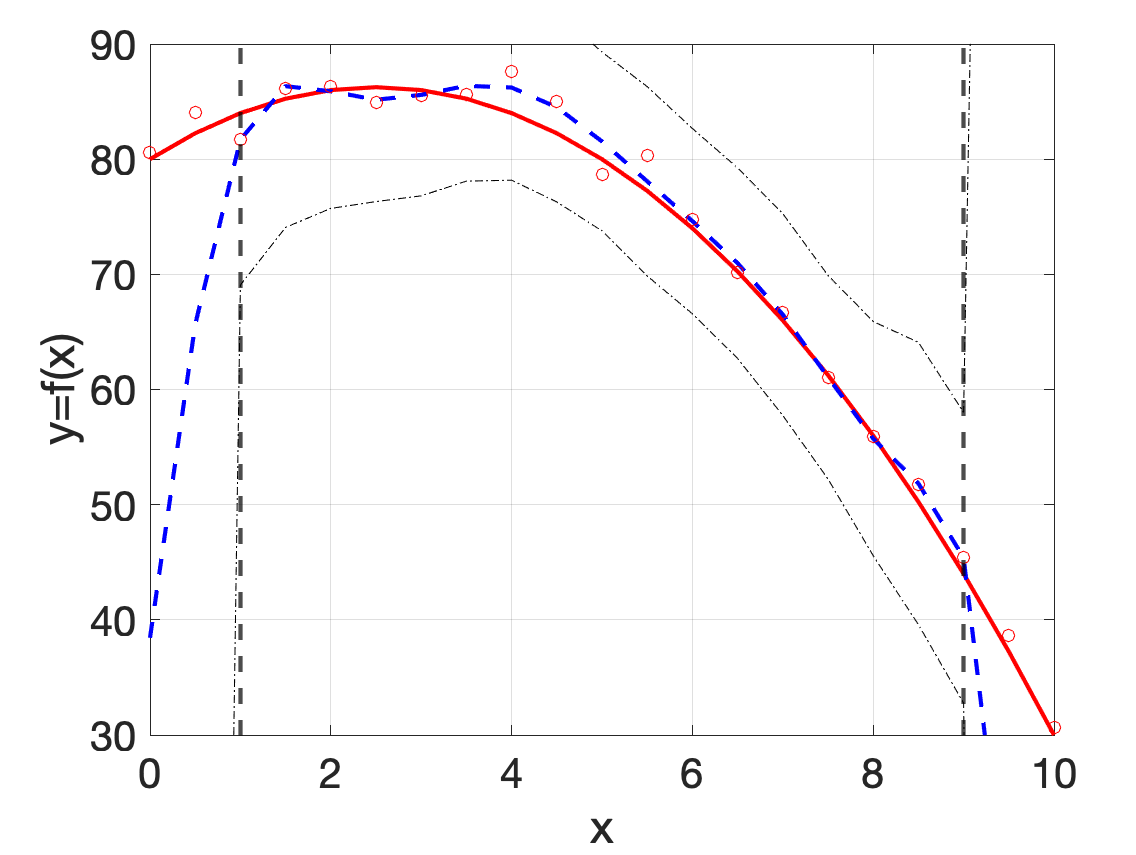
\includegraphics[width=0.7\linewidth]{sovra-b} \caption{}
			\end{subfigure}
			\caption{regressione di un campione di origine quadratica (linea rossa) tramite un polinomio di secondo grado (a) e di nono grado (b) rappresentati dalle linee tratteggiate blu.}
			\label{fig:stat:sovraadattamento}
		\end{figure}
	
\section{Taratura statica}
	La \de{taratura} di uno strumento di misura è l'identificazione della correlazione tra il misurando (il predittore $x$ della regressione) con l'uscita (risposta $y$) dello strumento stesso. La \de{taratura statica} è dunque effettuata in condizioni statiche, ossia assumendo che né misurando né uscita dello strumento siano funzioni del tempo, ma che siano costanti nello stesso.
	
	La correlazione $y=f(m)$ tra ingresso $m$ e uscita $y$ in condizioni statiche è detta \de{caratteristica statica} dello strumento. In generale uno strumento di misura operante in condizioni statiche fornisce una misura mediante l'inversione della caratteristica statica: nota infatti la caratteristica e il valore osservato dall'uscita $y_0$ è possibile ottenere per inversione la stima del misurando $m_0$.	
	
	\figura{5}{1.5}{tarstat-b}{stima del misurando ottenuta tramite inversione della caratteristica statica sfruttando l'uscita osservata dallo strumento.}{tarstat}
	
	Nella fase di \textbf{taratura} in generale la \textbf{caratteristica statica} è \textbf{ignota} ed è dunque necessario utilizzare una serie di valori noti del misurando $m_i$ per determinare le uscite attese $y_i$ in modo da \textit{costruire} la caratteristica statica del modello mediante un'opportuna regressione.
	
	\figura{5}{1.5}{tarstat}{determinazione della caratteristica statica come regressione di misurandi noti e rispettive uscite.}{tarstat}
	
	Durante la fase di taratura è necessario che i misurandi $m_i$ siano:
	\begin{itemize}
		\item dei \textbf{campioni di riferimento} fondamentali per la grandezza in esame (come per esempio un set di masse di valore noto);
		\item campioni/ingressi generici misurati con uno \textbf{strumento di riferimento}.
	\end{itemize}
	In entrambi i casi è necessario imporre che l'accuratezza del campione/strumento di riferimento sia di almeno un ordine di grandezza superiore rispetto all'accuratezza del sistema di misura da tarare.
	
	Con la fase di taratura è dunque possibile determinare sia la caratteristica statica del sistema, ma soprattutto l'incertezza della misura; in particolare nella fase di determinazione della caratteristica si trovano:
	\begin{itemize}
		\item lo sviluppo del modello dello strumento;
		\item la raccolta dei dati di taratura;
		\item l'analisi di regressione dei dati raccolti;
		\item la validazione della regressione mediante l'analisi dei residui.
	\end{itemize}
	Per quanto riguarda l'incertezza è necessario determinare le componenti:
	\begin{itemize}
		\item di incertezza sul modello;
		\item di incertezza sulla stima del misurando;
		\item di incertezza sulla curva di taratura.
	\end{itemize}
	
	\paragraph{Sviluppo del modello} Lo sviluppo del modello si basa sui principi di funzionamento dello strumento di misura, per questo è tipicamente analitico; esistono tuttavia modelli di origine numerica o semi-empirica.
	
	Un modello completo include, in generale, anche delle relazioni dovuti agli ingressi di disturbo (come per esempio le variazioni dovute alle temperatura) e di uscita sul sistema stesso; la differenza tra modello e realtà assume il nome di \de{incertezza di modello}.
	
	\figura{7}{0.66}{sisttar}{schema a blocchi di un sistema di misura}{sisttar}
	
	Considerando lo schema a blocchi di un sistema di misura in figura \ref{sisttar}, è possibile osservare che la misura è soggetta principalmente a due tipi di ingresso:
	\begin{itemize}
		\item l'\textbf{ingresso modificante} è un tipo di ingresso che influisce direttamente sul modello del sistema e dunque nella sua caratteristica statica. Sono degli ingressi più complessi da trattare e sono preponderanti quando il modello della misura è approssimato e non considera un effetto dominante (per esempio le variazioni di proprietà dovute alla temperatura) che possono comportare tarature errate; per limitare questo tipo di problema tendenzialmente si esegue una sequenza di test casualizzata (ossia non si incrementano gradualmente i campioni di riferimento, ripetendo misura più volte, ma si continua a cambiare casualmente il misurando, in modo da distribuire più uniformemente gli errori);
		\item l'\textbf{ingresso interferente} invece è dovuto ai disturbi casuali (tendenzialmente molto piccoli) che si sommano all'uscita del modello; essi possono essere ridotti in fase di taratura effettuando più test (in tempi diversi) a misurandi (ossia ingressi ad effetti dominanti) costanti, permettendo dunque di considerare tali fluttuazioni come distribuite normalmente per via del teorema del limite centrale: questa operazione prende il nome di \de{controllo statico}.
	\end{itemize}
	
	\textbf{VOLENDO SI PUò AGGIUNGERE ESEMPIO}
	
\section{Analisi di incertezza}
	Secondo la norma \texttt{UNI 4546} una \de{misura}, che rappresenta un parametro di un sistema considerato in un suo determinato stato, è composta da una triade di elementi: il \textbf{valore}	(nell'esempio che segue $35.2$), la sua \textbf{incertezza} ($0.1$) e l'\textbf{unità di misura} ($m$) associata alla misurazione nella forma
	\[ 35.2 \pm 0.1 m \]
	
	\paragraph{Incertezza  e GUM} Il concetto di \de{incertezza} è definito tramite la norma \texttt{UNI-CEI-ENV 13005} delle \de{GUM} (\textit{Guide to Uncertainty in Measurement}); questa normativa sostituisce il vocabolario precedente ridefinendo l'errore come \textbf{incertezza} e il valore vero con il termine \textbf{stima}.
	
	L'incertezza si riferisce solamente alla componente stocastica (casuale e non prevedibile) della misura. Per normativa infatti le componenti di deviazioni sistematica (gli ingressi interferenti laddove possibile) della misura devono essere corretti prima di riportare la misura stessa. Se tali effetti sono ignoti, allora essi possono essere considerati nella componente stocastica anche se il loro impatto risulterà essere maggiore (questa operazione è consentita solamente se, nella fase di taratura, si effettuano dei test casualizzati).
	
	L'\de{incertezza tipo} (\textit{standard uncertainty}) $u_x$ della variabile stocastica $x$ è definita come la deviazione standard del valor medio di $x$; ricordando dunque che $V(\ov x) = s_x^2/n$, allora è possibile osservare che l'incertezza tipo è definita come
	\begin{equation}
		u_x = \frac{s_x}{\sqrt n} = \sqrt{ \frac{\sum_{i=1}^n \big(x_i-\ov x\big)^2}{n(n-1)}}
	\end{equation}
	L'\de{incertezza relativa} $u_{x,\textrm{rel}}$ esprime invece l'incertezza come rapporto adimensionale tra incertezza tipo $u_x$ e valor medio campionario misurato (in modulo):
	\begin{equation}
		u_{x,\textrm{rel}} = \frac{u_x}{|\ov x|}
	\end{equation}
	\begin{nota}
		L'incertezza relativa è utilizzata tendenzialmente per confrontare valori di misurando molto differenti in quanto esprimono la deviazione standard in funzione del misurando stesso.
	\end{nota}
	In generale l'incertezza relativa $u_{x,\textrm{rel}}$ è molto piccola e si indica con una sola cifra significativa e si usano 3 notazioni principalmente: notazione scientifica ($7\cdot 10^{-5}$), parti per mille ($0.7 ^o/_{oo}$) o parti per milione ($70ppm$).
	
	\subsection{Intervalli di confidenza}
		In generale è utile esprimere l'incertezza come un intervallo all'interno del quale è probabile che ricada il valore atteso della popolazione da cui è estratto il campione dei valori di misura osservati: tale intervallo, analogo a come visto per la regressione (pag. \pageref{sec:stat:regrpred}), è detto \de{intervallo di confidenza} e la relativa probabilità associata è detta \de{livello di confidenza}.
		
		\vspace{3mm}
		Come visto a pagina \pageref{sec:stat:teststudent} tramite il test di student è possibile definire la statistica di test $t_0$ (che si distribuisce come una distribuzione T di Student) noto un campione $\langle x_i\rangle$ di media campionaria $\ov x$ e deviazione standard $s_x$ rispetto alla popolazione di valore atteso $\mu_0$ come
		\[ t_0 = \frac{\ov x - \mu_0}{s_x / \sqrt n} \backsim t_n\]
		
		Conoscendo la distribuzione della statistica di test $t_0$, allora la probabilità che la stessa ricada con una probabilità $1-\alpha$ (dove $\alpha$ è il $\pval$ della statistica) in tale distribuzione può essere determinata in funzione del quantile di probabilità $\alpha_2$ della T di Student di ordine $n$ indicato come $t_{n,\alpha/2}$:
		\begin{align*}
			P\left(-t_{n,\alpha/2} < \frac{|\ov x - \mu 0|}{s_x/\sqrt n} < t_{n,\alpha/2} \right) & = 1-\alpha  \\			
			\xrightarrow{s_{x}/\sqrt n \rightarrow u_x} \qquad P \Big(\ov x - t_{n,\alpha/2} u_x < \mu_0  < \ov x + t_{n,\alpha/2} u_x\Big) & = 1- \alpha
		\end{align*}
		
		E' dunque possibile affermare che l'intervallo di estremi $\ov x \pm t_{n,\alpha/2}u_x$ è proprio l'intervallo all'interno del quale ricade il valore atteso con un \textbf{livello di confidenza} pari a $1-\alpha$. \\
		Essendo $s_x /\sqrt n$ pari all'incertezza tipo e definendo il quantile $t_{n,\alpha/2} = k_n$ il \textbf{fattore di copertura} (dipendente dalla dimensione del campione $n$) è possibile definire l'\de{incertezza estesa} $U_x$ della misura come
		\[ U_x = t_{n,\alpha/2} \frac{ s_x}{\sqrt n} = k_n \, u_x\]
		
		Di fatto il fattore di copertura $k_n$ permette di stabilire di quanto debba essere moltiplicata l'incertezza tipo per avere un'affidabilità pari a $1-\alpha$ in funzione del numero di campioni $n$ analizzati e a tal fine si utilizza generalmente la funzione CDF.
		\begin{nota}
			Per un numero di campioni $n>20$ la distribuzione T di Student può essere approssimata ad una distribuzione normale e dunque si può utilizzare la sua CDF.	
		\end{nota}
		In tabella \ref{tab:stat:copertura} è possibile osservare per alcuni fattori di confidenza $k$ il livello di confidenza associato.
		\begin{SCtable}[1.5][bht]
			\centering
			\begin{tabular} {c | c}
				$\quad k \quad $ & copertura $= 2f_{cd,l}(k)-1$ \\ \hline
				1 & 68.27\% \\
				1.645 & 90\% \\
				1.960 & 95\% \\
				2 & 95.45\% \\
				2.576 & 99\% \\
				3 & 99.73\%
			\end{tabular}
			\caption{livello di confidenza associato al fattore di copertura $k$.} \label{tab:stat:copertura}
		\end{SCtable}
	
	\subsection*{Incertezza ex-post}
		L'incertezza sui dati può anche essere calcolata ex-post, ossia su dati ottenuti da un sistema di misura di cui è nota l'incertezza e viene espressa in \textbf{intervallo di predizione} (associato alla probabilità che le nuove osservazioni rientrino in tale fascia) e \textbf{intervallo di confidenza} (associato alla probabilità rispetto alla quale ci si attende che il valor atteso della popolazione ricada).
	
	\subsection{Incertezza tipo e incertezza estesa}
		Salvo diverse indicazioni per le misurazioni si utilizza l'\de{incertezza tipo}, ossia seguendo la dicitura
		\[ 27.5 \pm 0.1mm \]
		allora il termine $0.1$ è associato all'incertezza tipo $u_x = 0.1$. E' altresì possibile utilizzare l'\de{incertezza estesa} aggiungendo alla misura il livello di confidenza associato all'incertezza tipo riportata con una dicitura del tipo
		\[ 27.5\pm 0.1 mm \quad \textrm{con confidenza al 99\%} \]
	
	
	
	
	
	
	
	
	